\documentclass{article}
\usepackage[dblblindworkshop]{neurips_2025}
\workshoptitle{}

\usepackage[utf8]{inputenc}
\usepackage[T1]{fontenc}
\usepackage{hyperref}
\usepackage{url}
\usepackage{booktabs}
\usepackage{amsfonts}
\usepackage{nicefrac}
\usepackage{microtype}
\usepackage{xcolor}
\usepackage{graphicx}

\title{ArtifactGEN: High-Fidelity Synthesis of EEG Artifacts with WGAN-GP and Diffusion Models}

\author{
  Hritik Arasu \\
  Department of Behavior and Brain Sciences\\
  University of Texas at Dallas\\
  Richardson, TX 75080 \\
  \texttt{hritik.arasu@UTDallas.edu} \\
  \And
  Faisal R. Jahangiri \\
  Department of Behavior and Brain Sciences\\
  University of Texas at Dallas\\
  Richardson, TX 75080 \\
  \texttt{faisal.jahangiri@utdallas.edu} \\
}

%%%%%%%%%%%%%%%%%%%%%%%%%%%%%%%%%%%%%%%%%%%%%%%%%%%%%%%%%%%%

\begin{document}

\maketitle

\begin{abstract}
We present ArtifactGEN, an end-to-end, reproducible pipeline for synthesizing multi-channel EEG artifact windows conditioned on artifact type. Our system targets subject-wise splits derived from the TUH EEG corpus and supports two complementary generative paradigms: (i) a conditional Wasserstein GAN with gradient penalty and a projection discriminator for stable, label-aware synthesis \citep{gulrajani2017improved,miyato2018cgans}, and (ii) a denoising diffusion model using a 1D U-Net with FiLM conditioning and classifier-free guidance \citep{ho2020denoising,ho2022classifierfree}. The pipeline includes robust preprocessing, configurable normalization, and a modular evaluation suite spanning signal-level, feature-space (FID/KID/PRD) \citep{heusel2017gans,binkowski2018demystifying,sajjadi2018assessing}, and functional tasks (train-real/test-synth and vice versa, plus AugMix-style augmentation \citep{hendrycks2020augmix}). We release code, configuration files, and analysis notebooks to facilitate rigorous comparisons and future work on EEG artifact generation and augmentation.
\end{abstract}

%%%%%%%%%%%%%%%%%%%%%%%%%%%%%%%%%%%%%%%%%%%%%%%%%%%%%%%%%%%%


\section{Introduction}
Artifacts in electroencephalography (EEG)---such as muscle activity, eye movements, electrode noise, chewing, and shivering---pose a major challenge for automated analysis and downstream clinical applications. Synthetic artifact segments can support data augmentation, algorithm stress testing, and robustness benchmarking without additional human labeling. However, artifact synthesis requires models that respect signal morphology, spectral properties, and channel correlations while remaining label aware.

We introduce ArtifactGEN, a practical framework that combines a conditional WGAN-GP with projection discriminator and a denoising diffusion model tailored to 1D multi-channel time series. ArtifactGEN provides: (i) curated, subject-wise splits and preprocessing tailored to artifact windows; (ii) two strong conditional generators with complementary biases; and (iii) a comprehensive, reproducible evaluation protocol. Our contributions are:
\begin{itemize}
    \item A subject-wise pipeline to curate labeled artifact windows with robust normalization and fixed-length padding/truncation.
    \item A conditional WGAN-GP with projection discriminator for stable, label-aware synthesis \citep{gulrajani2017improved,miyato2018cgans}.
    \item A 1D diffusion model with FiLM conditioning and classifier-free guidance \citep{ho2020denoising,ho2022classifierfree}.
    \item A transparent evaluation suite spanning signal-level properties, feature-space distances (FID/KID/PRD) \citep{heusel2017gans,binkowski2018demystifying,sajjadi2018assessing}, and functional tests including AugMix-style augmentation \citep{hendrycks2020augmix}.
\end{itemize}

%%%%%%%%%%%%%%%%%%%%%%%%%%%%%%%%%%%%%%%%%%%%%%%%%%%%%%%%%%%%

\section{Background}


%%%%%%%%%%%%%%%%%%%%%%%%%%%%%%%%%%%%%%%%%%%%%%%%%%%%%%%%%%%%

\section{Related Work}
	extbf{Wasserstein GANs.} WGAN-GP stabilizes adversarial training by enforcing a soft 1-Lipschitz constraint via a gradient penalty \citep{gulrajani2017improved}. Label conditioning via projection in the discriminator improves fidelity and semantic control \citep{miyato2018cgans}.

	extbf{Diffusion models.} Denoising diffusion probabilistic models (DDPMs) learn to invert a fixed noising process and produce high-fidelity samples \citep{ho2020denoising}. Classifier-free guidance trades off diversity and fidelity without a separate classifier \citep{ho2022classifierfree}. We adopt a 1D U-Net backbone for time series inspired by U-Net-style architectures \citep{ronneberger2015u}.

	extbf{Evaluation of generative models.} Feature-space distances such as FID \citep{heusel2017gans} and KID \citep{binkowski2018demystifying}, and precision/recall curves for distributions \citep{sajjadi2018assessing} are standard for images; we adapt them by extracting features from an EEG artifact classifier. Robustness-oriented augmentation like AugMix \citep{hendrycks2020augmix} can quantify downstream utility of synthetic data.

%%%%%%%%%%%%%%%%%%%%%%%%%%%%%%%%%%%%%%%%%%%%%%%%%%%%%%%%%%%%


\section{Dataset and Preprocessing}
We work with EEG artifact segments originating from the Temple University Hospital EEG resources \citep{obeid2016temple}. Our curation enforces subject-wise splits to avoid leakage: 149 train, 32 validation, and 32 test subjects. We consider five artifact classes: Muscle, Eye movement, Electrode, Chewing, and Shiver. Windows are extracted at a fixed target length (e.g., 250 samples) and padded or truncated as needed. Two normalization strategies are supported: (i) per-window min-max to $[-1,1]$ for adversarial training and (ii) per-recording/channel z-score for diffusion. The repository includes metadata, class maps, and split manifests to reproduce these steps.

\begin{figure}[t]
    \centering
    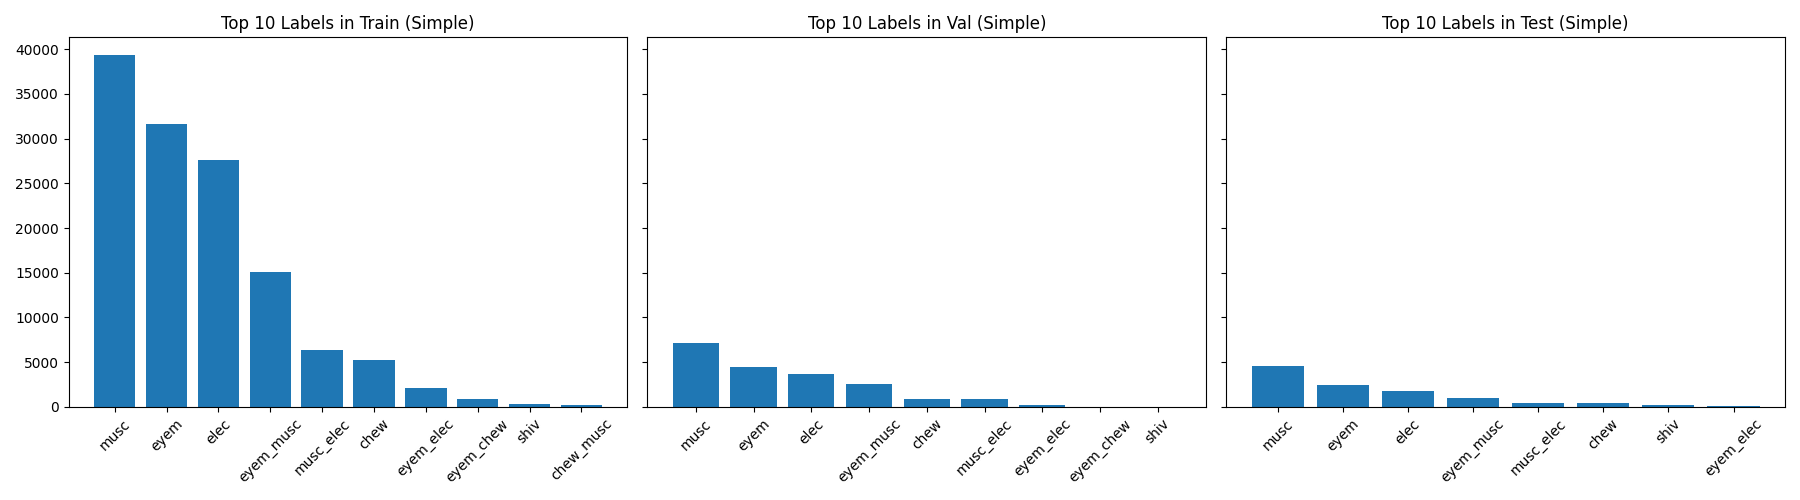
\includegraphics[width=.32\linewidth]{figs/label_dist_per_split_simple.png}\hfill
    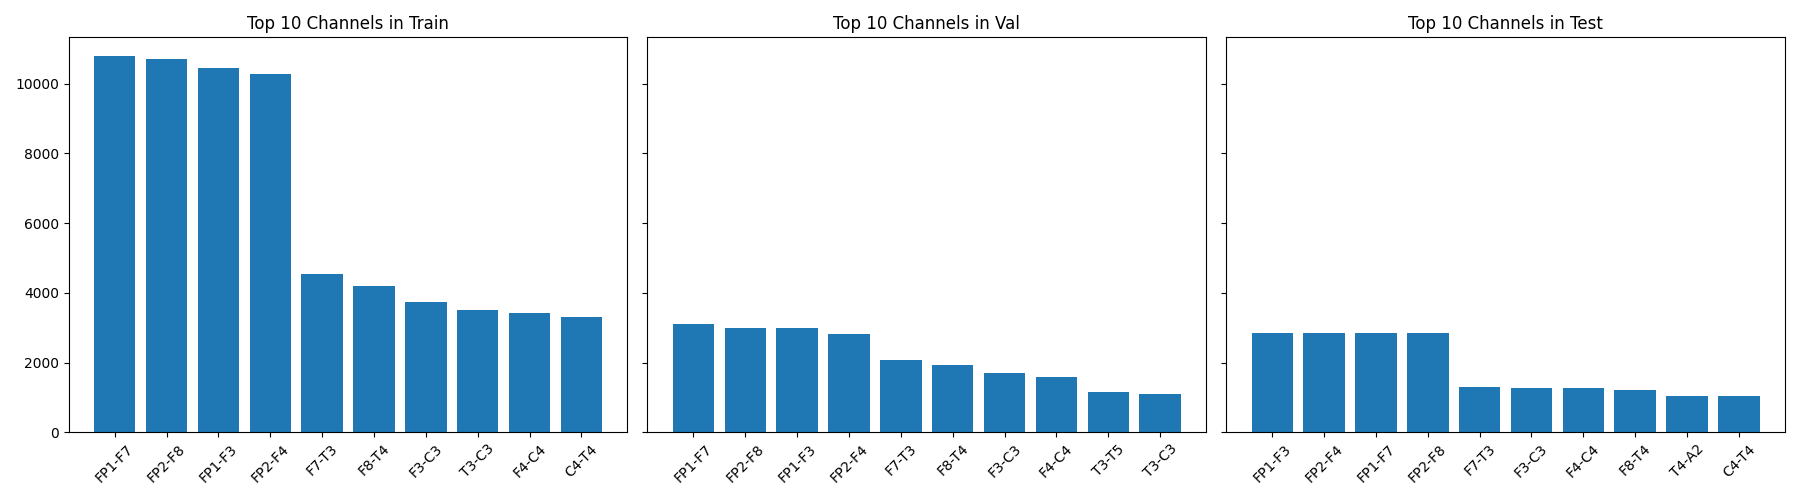
\includegraphics[width=.32\linewidth]{figs/channel_dist_per_split_multilabel.png}\hfill
    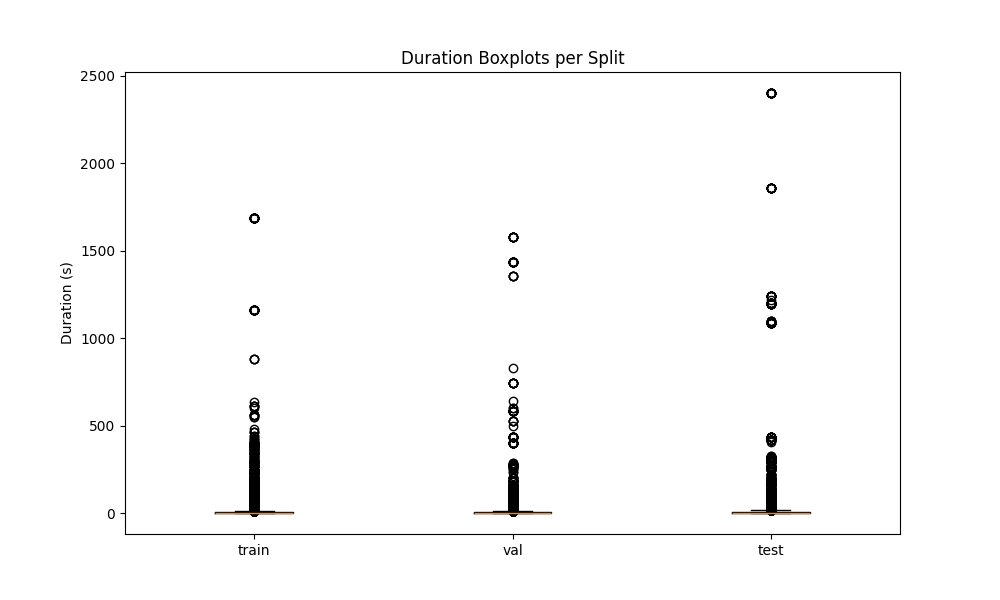
\includegraphics[width=.32\linewidth]{figs/duration_boxplot_multilabel.png}
    \caption{Data exploration: label distribution across splits, channel usage, and window duration statistics.}
\end{figure}

%%%%%%%%%%%%%%%%%%%%%%%%%%%%%%%%%%%%%%%%%%%%%%%%%%%%%%%%%%%%

\section{Methods}
\subsection{Conditional WGAN-GP with Projection Discriminator}
Our WGAN-GP uses a 1D transposed-convolutional generator that upsamples a concatenation of Gaussian noise and a one-hot class vector to multi-channel windows normalized to $[-1,1]$. The critic consists of strided 1D convolutions with global average pooling and a linear head. A projection term computes a dot product between learned class embeddings and critic features to produce class-aware scores \citep{miyato2018cgans}. Training minimizes the Wasserstein objective with gradient penalty \citep{gulrajani2017improved}. We optionally add an $L_1$ spectral loss between short-time Fourier transforms of real and synthetic signals to encourage frequency fidelity.

\subsection{Diffusion Model with 1D U-Net and FiLM Conditioning}
We implement DDPM with a 1D U-Net backbone, sinusoidal timestep embeddings, and FiLM layers that modulate intermediate features using a fused time-and-class conditioning vector. Labels are embedded, with a reserved null token to enable classifier-free guidance at sampling time \citep{ho2022classifierfree}. The network predicts noise in mean-squared error (MSE) training \citep{ho2020denoising}. Conditioning is applied at multiple resolutions with optional dilations to increase receptive field.

\subsection{Training}
All experiments are implemented in PyTorch \citep{paszke2019pytorch}. For WGAN-GP we use Adam \citep{kingma2015adam} for both generator and critic, $n_\text{critic}>1$, and a gradient penalty coefficient set via configuration. For DDPM we use AdamW \citep{loshchilov2019decoupled} and a linear beta schedule with $T$ steps. Early stopping monitors generator MSE or Wasserstein loss on the training stream; best checkpoints are saved automatically. TensorBoard logs track losses and, where enabled, spectral reconstruction.

\subsection{Evaluation}
	extbf{Signal-level.} We compute descriptive statistics (bandpower, spectra) and compare distributions between real and synthetic windows within each class.

	extbf{Feature-space.} We train a lightweight EEG artifact classifier on the training split and extract features to compute FID \citep{heusel2017gans}, KID \citep{binkowski2018demystifying}, and PRD curves \citep{sajjadi2018assessing} between real and synthetic sets, per class and overall.

	extbf{Functional.} We perform Train-Real/Test-Synth (TRTS) and Train-Synth/Test-Real (TSTR) classification to assess downstream utility, and evaluate AugMix-style augmentation where synthetic windows are mixed with real ones to test robustness \citep{hendrycks2020augmix}.

\begin{figure}[t]
    \centering
    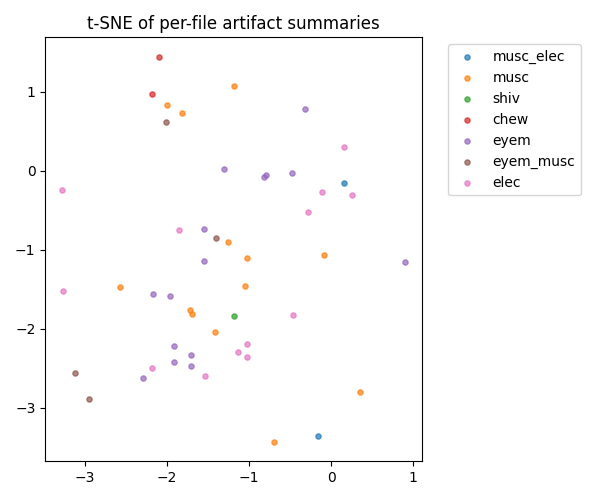
\includegraphics[width=.48\linewidth]{figs/tsne_perfile_summaries.png}\hfill
    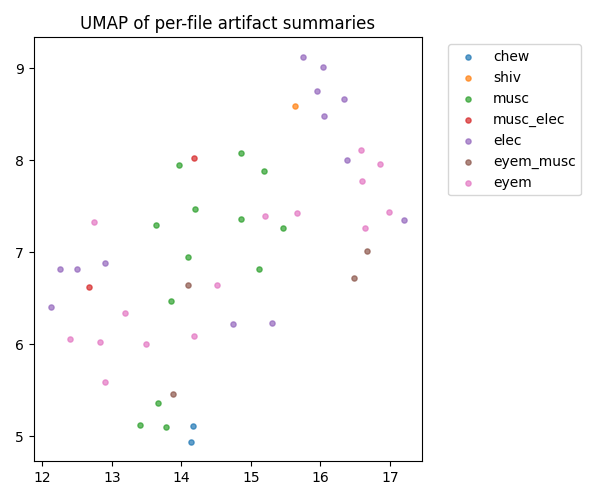
\includegraphics[width=.48\linewidth]{figs/umap_perfile_summaries.png}
    \caption{Low-dimensional embeddings (t-SNE \citep{maaten2008visualizing} and UMAP \citep{mcinnes2018umap}) of per-file artifact summaries illustrating separability and spread across classes.}
\end{figure}

%%%%%%%%%%%%%%%%%%%%%%%%%%%%%%%%%%%%%%%%%%%%%%%%%%%%%%%%%%%%

\section{Results}
Exploratory analysis confirms balanced subject-wise splits and class distributions. Qualitatively, both models produce diverse waveforms that respect per-class spectral characteristics; the optional spectral loss further aligns frequency content. Embedding plots of real vs. synthetic windows suggest good coverage without severe mode collapse. Full quantitative metrics (FID/KID/PRD) and TRTS/TSTR will be released with trained classifiers and checkpoints; our codebase contains the exact evaluation scripts and manifests to reproduce them.

%%%%%%%%%%%%%%%%%%%%%%%%%%%%%%%%%%%%%%%%%%%%%%%%%%%%%%%%%%%%
\section{Further Works}

\subsection{Limitations}
Our evaluation currently relies on a task-specific feature extractor rather than a universally standardized EEG embedding, which may bias FID/KID/PRD. The diffusion sampler adds computational overhead compared to the GAN. Finally, artifact definitions and channel montages vary across institutions; transfer may require reconditioning or fine-tuning.

\subsection{Ethics and Impact}
Synthetic EEG artifacts can reduce labeling burden and improve robustness testing for clinical and research pipelines. Misuse risks include over-reliance on synthetic data or distribution shift when deploying augmentation-trained models. We recommend releasing models with usage guidelines, reporting synthetic proportions, and validating on truly held-out subjects.

%%%%%%%%%%%%%%%%%%%%%%%%%%%%%%%%%%%%%%%%%%%%%%%%%%%%%%%%%%%%

\section{Conclusion}
ArtifactGEN provides a practical, reproducible foundation for EEG artifact synthesis with both WGAN-GP and diffusion models, plus a transparent evaluation suite. We hope this framework enables principled studies of augmentation, robustness, and generative modeling for EEG.


%%%%%%%%%%%%%%%%%%%%%%%%%%%%%%%%%%%%%%%%%%%%%%%%%%%%%%%%%%%%


\small
\bibliographystyle{plainnat}
\bibliography{CITATIONS}

\end{document}

%%%%%%%%%%%%%%%%%%%%%%%%%%%%%%%%%%%%%%%%%%%%%%%%%%%%%%%%%%%%
\newpage
\appendix

\section{Appendices and Supplementary Material}

%%%%%%%%%%%%%%%%%%%%%%%%%%%%%%%%%%%%%%%%%%%%%%%%%%%%%%%%%%%%

\clearpage
\section*{NeurIPS Paper Checklist}

\begin{enumerate}

\item {\bf Claims}
    \item[] Question: Do the main claims made in the abstract and introduction accurately reflect the paper's contributions and scope?
    \item[] Answer: \answerYes{}
    \item[] Justification: The abstract and introduction precisely state the method and the evaluation scope and they avoid broader clinical claims.
    \item[] Guidelines:
    \begin{itemize}
        \item The answer NA means that the abstract and introduction do not include the claims made in the paper.
        \item The abstract and/or introduction should clearly state the claims made, including the contributions made in the paper and important assumptions and limitations. A No or NA answer to this question will not be perceived well by the reviewers. 
        \item The claims made should match theoretical and experimental results, and reflect how much the results can be expected to generalize to other settings. 
        \item It is fine to include aspirational goals as motivation as long as it is clear that these goals are not attained by the paper. 
    \end{itemize}

\item {\bf Limitations}
    \item[] Question: Does the paper discuss the limitations of the work performed by the authors?
    \item[] Answer: \answerYes{}
    \item[] Justification: A dedicated Limitations paragraph notes dataset constraints (TUAR/TUEG only), potential covariate shift across sites/montages, limited ablations, and that downstream clinical utility is not established.
    \item[] Guidelines:
    \begin{itemize}
        \item The answer NA means that the paper has no limitation while the answer No means that the paper has limitations, but those are not discussed in the paper. 
        \item The authors are encouraged to create a separate "Limitations" section in their paper.
        \item The paper should point out any strong assumptions and how robust the results are to violations of these assumptions (e.g., independence assumptions, noiseless settings, model well-specification, asymptotic approximations only holding locally). The authors should reflect on how these assumptions might be violated in practice and what the implications would be.
        \item The authors should reflect on the scope of the claims made, e.g., if the approach was only tested on a few datasets or with a few runs. In general, empirical results often depend on implicit assumptions, which should be articulated.
        \item The authors should reflect on the factors that influence the performance of the approach. For example, a facial recognition algorithm may perform poorly when image resolution is low or images are taken in low lighting. Or a speech-to-text system might not be used reliably to provide closed captions for online lectures because it fails to handle technical jargon.
        \item The authors should discuss the computational efficiency of the proposed algorithms and how they scale with dataset size.
        \item If applicable, the authors should discuss possible limitations of their approach to address problems of privacy and fairness.
        \item While the authors might fear that complete honesty about limitations might be used by reviewers as grounds for rejection, a worse outcome might be that reviewers discover limitations that aren't acknowledged in the paper. The authors should use their best judgment and recognize that individual actions in favor of transparency play an important role in developing norms that preserve the integrity of the community. Reviewers will be specifically instructed to not penalize honesty concerning limitations.
    \end{itemize}

\item {\bf Theory assumptions and proofs}
    \item[] Question: For each theoretical result, does the paper provide the full set of assumptions and a complete (and correct) proof?
    \item[] Answer: \answerNA{}
    \item[] Justification: The paper is empirical and does not introduce new theorems or formal proofs; therefore no theoretical results or assumptions are claimed.
    \item[] Guidelines:
    \begin{itemize}
        \item The answer NA means that the paper does not include theoretical results. 
        \item All the theorems, formulas, and proofs in the paper should be numbered and cross-referenced.
        \item All assumptions should be clearly stated or referenced in the statement of any theorems.
        \item The proofs can either appear in the main paper or the supplemental material, but if they appear in the supplemental material, the authors are encouraged to provide a short proof sketch to provide intuition. 
        \item Inversely, any informal proof provided in the core of the paper should be complemented by formal proofs provided in appendix or supplemental material.
        \item Theorems and Lemmas that the proof relies upon should be properly referenced. 
    \end{itemize}

    \item {\bf Experimental result reproducibility}
    \item[] Question: Does the paper fully disclose all the information needed to reproduce the main experimental results of the paper to the extent that it affects the main claims and/or conclusions of the paper (regardless of whether the code and data are provided or not)?
    \item[] Answer: \answerYes{}
    \item[] Justification: We specify datasets, preprocessing, splits, model architecture, conditioning, loss/schedules, samplers, hyperparameters, seeds where applicable, and provide end-to-end commands in the supplement to reproduce figures and tables.
    \item[] Guidelines:
    \begin{itemize}
        \item The answer NA means that the paper does not include experiments.
        \item If the paper includes experiments, a No answer to this question will not be perceived well by the reviewers: Making the paper reproducible is important, regardless of whether the code and data are provided or not.
        \item If the contribution is a dataset and/or model, the authors should describe the steps taken to make their results reproducible or verifiable. 
        \item Depending on the contribution, reproducibility can be accomplished in various ways. For example, if the contribution is a novel architecture, describing the architecture fully might suffice, or if the contribution is a specific model and empirical evaluation, it may be necessary to either make it possible for others to replicate the model with the same dataset, or provide access to the model. In general. releasing code and data is often one good way to accomplish this, but reproducibility can also be provided via detailed instructions for how to replicate the results, access to a hosted model (e.g., in the case of a large language model), releasing of a model checkpoint, or other means that are appropriate to the research performed.
        \item While NeurIPS does not require releasing code, the conference does require all submissions to provide some reasonable avenue for reproducibility, which may depend on the nature of the contribution. For example
        \begin{enumerate}
            \item If the contribution is primarily a new algorithm, the paper should make it clear how to reproduce that algorithm.
            \item If the contribution is primarily a new model architecture, the paper should describe the architecture clearly and fully.
            \item If the contribution is a new model (e.g., a large language model), then there should either be a way to access this model for reproducing the results or a way to reproduce the model (e.g., with an open-source dataset or instructions for how to construct the dataset).
            \item We recognize that reproducibility may be tricky in some cases, in which case authors are welcome to describe the particular way they provide for reproducibility. In the case of closed-source models, it may be that access to the model is limited in some way (e.g., to registered users), but it should be possible for other researchers to have some path to reproducing or verifying the results.
        \end{enumerate}
    \end{itemize}


\item {\bf Open access to data and code}
    \item[] Question: Does the paper provide open access to the data and code, with sufficient instructions to faithfully reproduce the main experimental results, as described in supplemental material?
    \item[] Answer: \answerYes{}
    \item[] Justification: Data is public (TUAR/TUEG) and paper contains pointers and preparation steps so others can recreate our pipelines.
    \item[] Guidelines:
    \begin{itemize}
        \item The answer NA means that paper does not include experiments requiring code.
        \item Please see the NeurIPS code and data submission guidelines (\url{https://nips.cc/public/guides/CodeSubmissionPolicy}) for more details.
        \item While we encourage the release of code and data, we understand that this might not be possible, so “No” is an acceptable answer. Papers cannot be rejected simply for not including code, unless this is central to the contribution (e.g., for a new open-source benchmark).
        \item The instructions should contain the exact command and environment needed to run to reproduce the results. See the NeurIPS code and data submission guidelines (\url{https://nips.cc/public/guides/CodeSubmissionPolicy}) for more details.
        \item The authors should provide instructions on data access and preparation, including how to access the raw data, preprocessed data, intermediate data, and generated data, etc.
        \item The authors should provide scripts to reproduce all experimental results for the new proposed method and baselines. If only a subset of experiments are reproducible, they should state which ones are omitted from the script and why.
        \item At submission time, to preserve anonymity, the authors should release anonymized versions (if applicable).
        \item Providing as much information as possible in supplemental material (appended to the paper) is recommended, but including URLs to data and code is permitted.
    \end{itemize}


\item {\bf Experimental setting/details}
    \item[] Question: Does the paper specify all the training and test details (e.g., data splits, hyperparameters, how they were chosen, type of optimizer, etc.) necessary to understand the results?
    \item[] Answer: \answerYes{}
    \item[] Justification: The Methods and Appendix enumerate data splits, montage, sampling rate, optimizer/schedule, diffusion steps/sampler, batch size, conditioning scheme, and selection rationales.
    \item[] Guidelines:
    \begin{itemize}
        \item The answer NA means that the paper does not include experiments.
        \item The experimental setting should be presented in the core of the paper to a level of detail that is necessary to appreciate the results and make sense of them.
        \item The full details can be provided either with the code, in appendix, or as supplemental material.
    \end{itemize}

\item {\bf Experiment statistical significance}
    \item[] Question: Does the paper report error bars suitably and correctly defined or other appropriate information about the statistical significance of the experiments?
    \item[] Answer: \answerNo{}
    \item[] Justification: Current results report point estimates across runs/partitions without CIs; we note this and plan to include bootstrap CIs and seed variance in a revision.
    \item[] Guidelines:
    \begin{itemize}
        \item The answer NA means that the paper does not include experiments.
        \item The authors should answer "Yes" if the results are accompanied by error bars, confidence intervals, or statistical significance tests, at least for the experiments that support the main claims of the paper.
        \item The factors of variability that the error bars are capturing should be clearly stated (for example, train/test split, initialization, random drawing of some parameter, or overall run with given experimental conditions).
        \item The method for calculating the error bars should be explained (closed form formula, call to a library function, bootstrap, etc.)
        \item The assumptions made should be given (e.g., Normally distributed errors).
        \item It should be clear whether the error bar is the standard deviation or the standard error of the mean.
        \item It is OK to report 1-sigma error bars, but one should state it. The authors should preferably report a 2-sigma error bar than state that they have a 96\% CI, if the hypothesis of Normality of errors is not verified.
        \item For asymmetric distributions, the authors should be careful not to show in tables or figures symmetric error bars that would yield results that are out of range (e.g. negative error rates).
        \item If error bars are reported in tables or plots, The authors should explain in the text how they were calculated and reference the corresponding figures or tables in the text.
    \end{itemize}

\item {\bf Experiments compute resources}
    \item[] Question: For each experiment, does the paper provide sufficient information on the computer resources (type of compute workers, memory, time of execution) needed to reproduce the experiments?
    \item[] Answer: \answerYes{}
    \item[] Justification: Appendix provides environment details
    \item[] Guidelines:
    \begin{itemize}
        \item The answer NA means that the paper does not include experiments.
        \item The paper should indicate the type of compute workers CPU or GPU, internal cluster, or cloud provider, including relevant memory and storage.
        \item The paper should provide the amount of compute required for each of the individual experimental runs as well as estimate the total compute. 
        \item The paper should disclose whether the full research project required more compute than the experiments reported in the paper (e.g., preliminary or failed experiments that didn't make it into the paper). 
    \end{itemize}
    
\item {\bf Code of ethics}
    \item[] Question: Does the research conducted in the paper conform, in every respect, with the NeurIPS Code of Ethics \url{https://neurips.cc/public/EthicsGuidelines}?
    \item[] Answer: \answerYes{}
    \item[] Justification: We use de-identified, publicly available EEG datasets under their licenses.
    \item[] Guidelines:
    \begin{itemize}
        \item The answer NA means that the authors have not reviewed the NeurIPS Code of Ethics.
        \item If the authors answer No, they should explain the special circumstances that require a deviation from the Code of Ethics.
        \item The authors should make sure to preserve anonymity (e.g., if there is a special consideration due to laws or regulations in their jurisdiction).
    \end{itemize}


\item {\bf Broader impacts}
    \item[] Question: Does the paper discuss both potential positive societal impacts and negative societal impacts of the work performed?
    \item[] Answer: \answerYes{}
    \item[] Justification: We outline benefits and risks with mitigation notes.
    \item[] Guidelines:
    \begin{itemize}
        \item The answer NA means that there is no societal impact of the work performed.
        \item If the authors answer NA or No, they should explain why their work has no societal impact or why the paper does not address societal impact.
        \item Examples of negative societal impacts include potential malicious or unintended uses (e.g., disinformation, generating fake profiles, surveillance), fairness considerations (e.g., deployment of technologies that could make decisions that unfairly impact specific groups), privacy considerations, and security considerations.
        \item The conference expects that many papers will be foundational research and not tied to particular applications, let alone deployments. However, if there is a direct path to any negative applications, the authors should point it out. For example, it is legitimate to point out that an improvement in the quality of generative models could be used to generate deepfakes for disinformation. On the other hand, it is not needed to point out that a generic algorithm for optimizing neural networks could enable people to train models that generate Deepfakes faster.
        \item The authors should consider possible harms that could arise when the technology is being used as intended and functioning correctly, harms that could arise when the technology is being used as intended but gives incorrect results, and harms following from (intentional or unintentional) misuse of the technology.
        \item If there are negative societal impacts, the authors could also discuss possible mitigation strategies (e.g., gated release of models, providing defenses in addition to attacks, mechanisms for monitoring misuse, mechanisms to monitor how a system learns from feedback over time, improving the efficiency and accessibility of ML).
    \end{itemize}
    
\item {\bf Safeguards}
    \item[] Question: Does the paper describe safeguards that have been put in place for responsible release of data or models that have a high risk for misuse (e.g., pretrained language models, image generators, or scraped datasets)?
    \item[] Answer: \answerNA{}
    \item[] Justification: The released assets (training code and small domain-specific models) are not high-risk general-purpose generators; we nevertheless include usage notes and disclaimers but no gated access is required.
    \item[] Guidelines:
    \begin{itemize}
        \item The answer NA means that the paper poses no such risks.
        \item Released models that have a high risk for misuse or dual-use should be released with necessary safeguards to allow for controlled use of the model, for example by requiring that users adhere to usage guidelines or restrictions to access the model or implementing safety filters. 
        \item Datasets that have been scraped from the Internet could pose safety risks. The authors should describe how they avoided releasing unsafe images.
        \item We recognize that providing effective safeguards is challenging, and many papers do not require this, but we encourage authors to take this into account and make a best faith effort.
    \end{itemize}

\item {\bf Licenses for existing assets}
    \item[] Question: Are the creators or original owners of assets (e.g., code, data, models), used in the paper, properly credited and are the license and terms of use explicitly mentioned and properly respected?
    \item[] Answer: \answerYes{}
    \item[] Justification: We cite the data sources used as well as the packages.
    \item[] Guidelines:
    \begin{itemize}
        \item The answer NA means that the paper does not use existing assets.
        \item The authors should cite the original paper that produced the code package or dataset.
        \item The authors should state which version of the asset is used and, if possible, include a URL.
        \item The name of the license (e.g., CC-BY 4.0) should be included for each asset.
        \item For scraped data from a particular source (e.g., website), the copyright and terms of service of that source should be provided.
        \item If assets are released, the license, copyright information, and terms of use in the package should be provided. For popular datasets, \url{paperswithcode.com/datasets} has curated licenses for some datasets. Their licensing guide can help determine the license of a dataset.
        \item For existing datasets that are re-packaged, both the original license and the license of the derived asset (if it has changed) should be provided.
        \item If this information is not available online, the authors are encouraged to reach out to the asset's creators.
    \end{itemize}

\item {\bf New assets}
    \item[] Question: Are new assets introduced in the paper well documented and is the documentation provided alongside the assets?
    \item[] Answer: \answerNA{}.
    \item[] Justification: Did not provide any additional code apart from the instructions given.
    \item[] Guidelines:
    \begin{itemize}
        \item The answer NA means that the paper does not release new assets.
        \item Researchers should communicate the details of the dataset/code/model as part of their submissions via structured templates. This includes details about training, license, limitations, etc. 
        \item The paper should discuss whether and how consent was obtained from people whose asset is used.
        \item At submission time, remember to anonymize your assets (if applicable). You can either create an anonymized URL or include an anonymized zip file.
    \end{itemize}

\item {\bf Crowdsourcing and research with human subjects}
    \item[] Question: For crowdsourcing experiments and research with human subjects, does the paper include the full text of instructions given to participants and screenshots, if applicable, as well as details about compensation (if any)? 
    \item[] Answer: \answerNA{}.
    \item[] Justification: No new human-subjects data or crowdsourcing were conducted; we rely solely on public de-identified datasets.
    \item[] Guidelines:
    \begin{itemize}
        \item The answer NA means that the paper does not involve crowdsourcing nor research with human subjects.
        \item Including this information in the supplemental material is fine, but if the main contribution of the paper involves human subjects, then as much detail as possible should be included in the main paper. 
        \item According to the NeurIPS Code of Ethics, workers involved in data collection, curation, or other labor should be paid at least the minimum wage in the country of the data collector. 
    \end{itemize}

\item {\bf Institutional review board (IRB) approvals or equivalent for research with human subjects}
    \item[] Question: Does the paper describe potential risks incurred by study participants, whether such risks were disclosed to the subjects, and whether Institutional Review Board (IRB) approvals (or an equivalent approval/review based on the requirements of your country or institution) were obtained?
    \item[] Answer: \answerNA{}
    \item[] Justification: The work analyzes public, de-identified EEG datasets and does not involve direct human-subjects research requiring IRB review for this study.
    \item[] Guidelines:
    \begin{itemize}
        \item The answer NA means that the paper does not involve crowdsourcing nor research with human subjects.
        \item Depending on the country in which research is conducted, IRB approval (or equivalent) may be required for any human subjects research. If you obtained IRB approval, you should clearly state this in the paper. 
        \item We recognize that the procedures for this may vary significantly between institutions and locations, and we expect authors to adhere to the NeurIPS Code of Ethics and the guidelines for their institution. 
        \item For initial submissions, do not include any information that would break anonymity (if applicable), such as the institution conducting the review.
    \end{itemize}

\item {\bf Declaration of LLM usage}
    \item[] Question: Does the paper describe the usage of LLMs if it is an important, original, or non-standard component of the core methods in this research? Note that if the LLM is used only for writing, editing, or formatting purposes and does not impact the core methodology, scientific rigorousness, or originality of the research, declaration is not required.
    %this research? 
    \item[] Answer: \answerNA{}
    \item[] Justification: LLMs are not part of the core technical method; any editorial assistance does not impact the scientific methodology and thus does not require declaration.
    \item[] Guidelines:
    \begin{itemize}
        \item The answer NA means that the core method development in this research does not involve LLMs as any important, original, or non-standard components.
        \item Please refer to our LLM policy (\url{https://neurips.cc/Conferences/2025/LLM}) for what should or should not be described.
    \end{itemize}

\end{enumerate}

\end{document}